\documentclass[aspectratio=169, 12pt, final]{beamer}
\usepackage{caption}
\captionsetup[table]{labelformat=empty}
\usepackage{graphicx}

\setbeamertemplate{navigation symbols}{}
\setbeamertemplate{caption}[numbered]

\usepackage[utf8]{inputenc}
\usepackage{enumerate}
\usepackage{tikz}
\usepackage{adjustbox}
\usepackage{marvosym}

\usetheme{default}


\usefonttheme[onlymath]{serif}%makes the math look right;

\usepackage{graphicx}
\usepackage{overpic}
\usepackage{transparent}
\usepackage{multirow}
\usepackage{colortbl}
%\usepackage[eurosym]{eurofont}
\usepackage{caption}
%\usepackage[table]{xcolor}
\usepackage[font=scriptsize,labelfont=bf]{caption}
\usepackage{sidecap}
\usepackage{booktabs}


%\DeclareCaptionFont{blue}{\color{blue}}
%\captionsetup{labelfont={blue,bf}}
\usepackage{booktabs}
\usepackage{centernot}


\title{Buffalo Hunt: International Trade and the Virtual Extinction of the North American Bison \\
M. Scott Taylor (2011, AER)}
\author{Jeanne Sorin}
\date{October 29, 2020}




\begin{document}

\frame{\titlepage}

\iffalse
Slide 2

Historical context
Split in 2 parts
Subsistence hunting by Natives and Settlers
Habitat destruction: building of the Pacific Railroad through the Platte River Valley in the 1860s
Different scale
2 periods
\fi


% This may be overly familiar to you, but let's still put the "slaughter of the american bison" into historical perspective. 
% We estimate that there were 25 to 30 million Buffalos (or american bison) in North American in the 16th century.
% We can split the decrease in the population into two parts. The first part covers the first half of the XIXth century, up until the beggining of the 1870s and witnessed the extinction of Buffalos at the east of the Mississipi by 1830s, and continued westwards towards the Great Plains. 
%Bisons were hunt both by Natives and Settlers in what is commonly acknowledged to be subsistence hunting, and also suffered from habitat destruction. One can for example mention the building of the Union Pacific Railroad through the Platte River Valley in the 1860s. 
% We estimate that in 1865, between 10 and 15 million Buffalos remained.
% What happens next is on a totally different scale, in terms of pace as, within 20 years, the population dropped to 100 bisons in the Great Plains States. During this period we can distinguish 2 phases, a first one in the seventies where the buffalo was hunt in the Southern Great Plains, and then in eighties when the buffalo was hunt in the Northern Great Plains.

% So what happened during this 20 years period? And why is this important today? Not only from a historical perspective, but also from an economics and especially resource economics and policy perspectives?

\begin{frame}
\frametitle{What happened to the American Bison? - The Timeline}
\begin{columns}
\begin{column}{0.7\textwidth}
\footnotesize{
\begin{itemize}
	\item \textbf{16th century}: 25 to 30 million Buffalos in North America
	%\item \textbf{Before 1830}: Buffalos removed at the east of the Mississipi
	\begin{itemize}
		\item Habitat destruction, subsistence hunting %as settlers were moving westwards
	\end{itemize}
	%\item \textbf{1860s}: The Union Pacific Railroad 
	\item \textbf{1865}: 10 to 15 million Buffalos remaining
	\pause
	\item \textbf{1870-1871}: Tanning innovation in Europe %shift where Buffalo hides are considered as a valuable commodity
		% How going from meat to hide gets makes it valuable to kill everywhere as there isn't this écloseness" constraint : you don't need to hide to stay fresh, unless the meat.
	\item \textbf{1872-1879}: Buffalo hunt in the Southern Great Plains
	\item \textbf{1881-1886}: Buffalo hunt in the Northern Great Plains 
	\item \textbf{1886}: 100 Buffalos remaining in the Great Plains States.
\end{itemize}	
}
\end{column}
\begin{column}{0.3\textwidth}
		
\includegraphics[width=1\textwidth]{photo.png}
\end{column}	
\end{columns}
\end{frame}

\iffalse
Classical explanation = continuation + intensification
International story : tanning innovation Europe 1870-1871
Bisons more valuable
Exponential increase in hunting
Combination of 3 necessary and sufficient conditions

May tell me: what about causality —> exploit the angle of the rate of the slaughter to tie resource overuse to trade
\fi


% The classical explanation for what happened during this second phase, is a continuation of what happened during the first half of the 19th century, but with an increase in hunting due to railroad workers hunting bisons as the Union Pacific was spreading, accompanied by hunting by the US army, as well as the intensification of hunting by the natives.
% This very american story is not, however, the one retained by the author who believes and argues that the exinction of the american bison actually is an international history or more preciselt, a European-American history.
% Indeed he makes the case it is a tanning innovation in Europe in 1870-1871, passed on to the US through international trade, that caused this ecological catastrophe: because of tanning, the meat of the bison was not the only valuable part anymore, and because the hide is not perishable, bison hunting is much less constrained by transport and close demand, leading to an exponential increase in hunting.
% More precisely, he argues that there is a combination of 3 necessary and sufficient conditions for the Buffalo slaughter :
% 1. 
% 2.
% 3.

%At that point you may tell me, well, this is an interesting hypothesis, but how do you go on establishing the causality? This is, I think, one of the main contribution of this paper, as it exploits an angle, the rate of the slaughter, that is used to tie resource overuse to trade, which is usually really hard to do, because all endogeneity and confounding factors issues.
%Focusing on the rate of the slaughter, Taylor tries to establish the causality of the tanning innovation by first developing a simple model of Buffalo Hunting, documenting extensively the assumptions needed for his model to apply to the slaughter, and by conducting the empirical analysis of a quasi-experiment.

\begin{frame}
\frametitle{What happened to the American Bison? - The Hypotheses}	
\begin{itemize}
	\item \textbf{Classical candidates} : railroads, US Army, changes in native hunting practices
\item \textbf{A new hypothesis}: the key role of international trade
\begin{itemize}
	\item Necessary and sufficient explanations of the Buffalo slaughter
	\begin{enumerate}
		\item A price for buffalo products that was largely invariant to changes in supply
		\item Open access conditions with no regulation of the buffalo kill
		\item A newly invented tanning process that allowed buffalo hides to be turned into valuable commercial leather
	\end{enumerate}
	\item Lever: focusing on a the rate of the slaughter
	\begin{enumerate}
		\item A simple Model of Buffalo Hunting
		\item A newly constructed export data
		\item Empirical Analysis 
	\end{enumerate}
\end{itemize}
\end{itemize}
\end{frame}






% Obviously, this research would already be valuable from a pure historical account perspective, but as I just mentioned it is also important from an economics, and especially a resource economics perspective.
% A key contribution of this paper is to establish how resource overuse can be tied to trade, in this case how trade galvanized resource overuse (and I will detail what I mean exactly by resource overuse when going over the model).
% Another major contribution is to link this catastrophe to the absence of property rights on bisons, and suggest explanations why these property rights did not arise. 
% In the same veine as Lueck and Benson, Taylor seems to argue that market forces provided incentives against property rights: because domestication was too costly, or because the high price and free entry gave the market a lot of leverage.
% More generally, the impact of market forces on the depletion of renewable resources is something that is studied a lot, in the contemporary context, but that has also been studied a lot by economic historians:
% - Ann M. Carlos and Frank D. Lewis (1993, 1999) --> depletion of beaver in 18th century
% - Patterson and Wilen (1977) --> northern pacific seal hunt
% - Robert C. All and Ian Keay (2004), who study the extinction of the Artic Bowhead Whale.
% Naturally, this brings the question of why institutions did not adapt, or not fast enough. Indeed, when we talk about property rights, as did Coase in the other of today's readings, we cannot abstract from discussing the role of institutions. 
% This is especially important nowadays as many developing countries in the world rely heavily on resource exports and very few have strong regulations governing resource use.



\begin{frame}
\frametitle{Why should we care? - An Economics Perspective}	
\begin{itemize}
	\item Historical Account
	\item Resource Economics
	\begin{itemize}
		\item Trade as galvanizing force of market failues
		\item (Absence of) property rights and institution adaptation
		\begin{itemize}
			\item Fixed price for Bison limiting economic incentives for regulation and preventing scarcity signals
			\item \textcolor{blue}{D. Lueck (2002) ; B. Benson (2006)}
		\end{itemize}
		\item Market forces and the depletion of renewable resources
		\begin{itemize}
			\item \textcolor{blue}{A.M. Carlos and F.D. Lewis (1993, 1999) ; Patterson and Wilen (1977) ; \\R.C. All and I. Keay (2004)}
		\end{itemize}
	\end{itemize}
	\item Policy
	\begin{itemize}
		\item Developing countries relying on resource exports and pressured by globalization
	\end{itemize}
\end{itemize}
\end{frame}



% Now, before jumping into the model, and the empirical analysis etcaetera, I would like to take a minute just to reflect on what Taylor's approach is here.
%He defined, let me go back one slide, three necessary and sufficient conditions for the Buffalo slaughter. The "necessary and sufficient" adjectives are important because they, together, will imply the causal mechanism that economists are always looking for.
%First, in order to prove that these three conditions are sufficient, Taylor will develop a simple theoretical model of Buffalo hunting showing that these three elements deliver a punctuated slaughter, that matches the one of the Great Plains. In a second time, to prove necessity, he will move to the empirical analysis. 
% So let's look at the sufficiency bit first.

% Taylor develops a simple dynamic model where agents hunt for buffalo or work in the outside good sector, where they get the wage w. Hunters differ in their hunting skills \alpha, and have a net productivity of \alpha times S(t), where S(t) is the size of the Buffalo Herd. p is the price they get for a Buffalo.
%Note that the hunter's payoff is increasing in \alpha, so there is a marginal \alpha^* below which it's more profitable to work in the outside sector. So all workers with \alpha above \alpha^* will hunt and all workers with \alpha below \alpha^* will work in the outside sector

% As we are looking at a dynamic problem, we need to specify the LOM for the Herd, that is the biological growth G(s) of the Herd, minus the killing per unit of time K.
% This killing per unit of time is called the resource constraint by Taylor and accounts for the number of workers (N times the cumulatve density of all individuals with alpha above alpha^*, times the productivity of these workers. 

%From a dynamic programming perspective, alpha^* and S are the state variables, while the choice variable is whether to hunt or not (discrete problem here), p is an exogenous parameter. Therefore, this model captures the fact that entry and exit into hunting is endogenous !

% Is there any question ?

\begin{frame}
\frametitle{Proving Sufficiency Through a Model - Setup}
\begin{itemize}
	\item \textbf{The Hunter's problem}  : $\max \{\underbrace{p \cdot h = p \cdot \alpha \cdot S(t)}_{\text{Hunting}} ; \underbrace{w = 1}_{\text{Outside option, numeraire}} \}$.
\\ 
\footnotesize{$\alpha$ hunter's hunting skills $\sim F(\alpha)$} ; $\alpha^*$ marginal hunter
%$\Rightarrow$ \textbf{Marginal hunter} s.t. $ p \cdot \alpha^{*} \cdot S(t) = w$
\item  \textbf{Buffalo Herd $S(t)$ Growth LOM:} 
 \begin{align*}
 	\dot{S} &= \underbrace{G(S)}_{\text{Biological Growth }} - K(p, S) \\
 	& G'(S) > 0 ; G''(S) \leq 0 ; G(0) = 0
 \end{align*}
\item \textbf{Resource constraint} 
\begin{align*}
 	\underbrace{\bar{K}(\alpha^*, S)}_{\text{\# buffalo killed}} &= \underbrace{N\cdot \int_{\alpha^*}^{\bar{\alpha}} f(\alpha)}_{\text{\# hunters}} \underbrace{S \cdot \alpha}_{\text{productivity}} d\alpha
 \end{align*} 
  \begin{align*}
 	\frac{d K(p,s)}{dS} &= N \int_{\alpha^*}^{\bar{\alpha}} \alpha f(\alpha) d\alpha - NS \alpha^* f(\alpha^*) \underbrace{\frac{d \alpha^*}{dS}}_{< 0} > 0
 \end{align*}
\end{itemize}
\end{frame}

%LHS = number of buffalo killed per unit of time when the herd is of size S and agents of productivity greated than star engaged in the hunting. \\
%RHS : $f(\alpha)$ density of agents with $\alpha$, $\alpha S$ productivity ; $N$ share of these.
%$N[1 - F(\alpha^*)]$ number of active hunters ; $N[F(\alpha^*]$ number of outside workers.




% With C being the maximum Herd size (without killing), and S_s the minimum herd size at which it is profitable for at least one hunter (with the maximum alpha) to hunt rather than work in the outside sector, this model features a unique interior steady state S^*

% How does this model, and this graph work: at time t, when people start killing bisons, we are on the K path, which is also the killing function (the same way that in other resource extraction models, y is both the production rate and the stock depletion rate). As we kill bison, we move down the K path.
% and you can think of the time before that as a time where hunting bison skills were too low to have even one bison hunter.

\begin{frame}
\frametitle{Proving Sufficiency Through a Model - Steady State}
\begin{columns}
\begin{column}{0.6\textwidth}
\footnotesize{
\textbf{Proposition}: Assume $C > S_s$, then there exists}
\begin{enumerate}[(i)]
 	\item \footnotesize{a unique interior steady state herd size $S^* \in [S_s, C]$}
 	\item \footnotesize{a unique marginal hunter $\alpha^*(p, S^*) \in (0, \bar{\alpha})$}
 	\item \footnotesize{starting from any $S > 0$, convergence to $S^*$ is monotonic}
 \end{enumerate}
\end{column}
\begin{column}{0.5\textwidth}  %%<--- here
    \begin{center}
     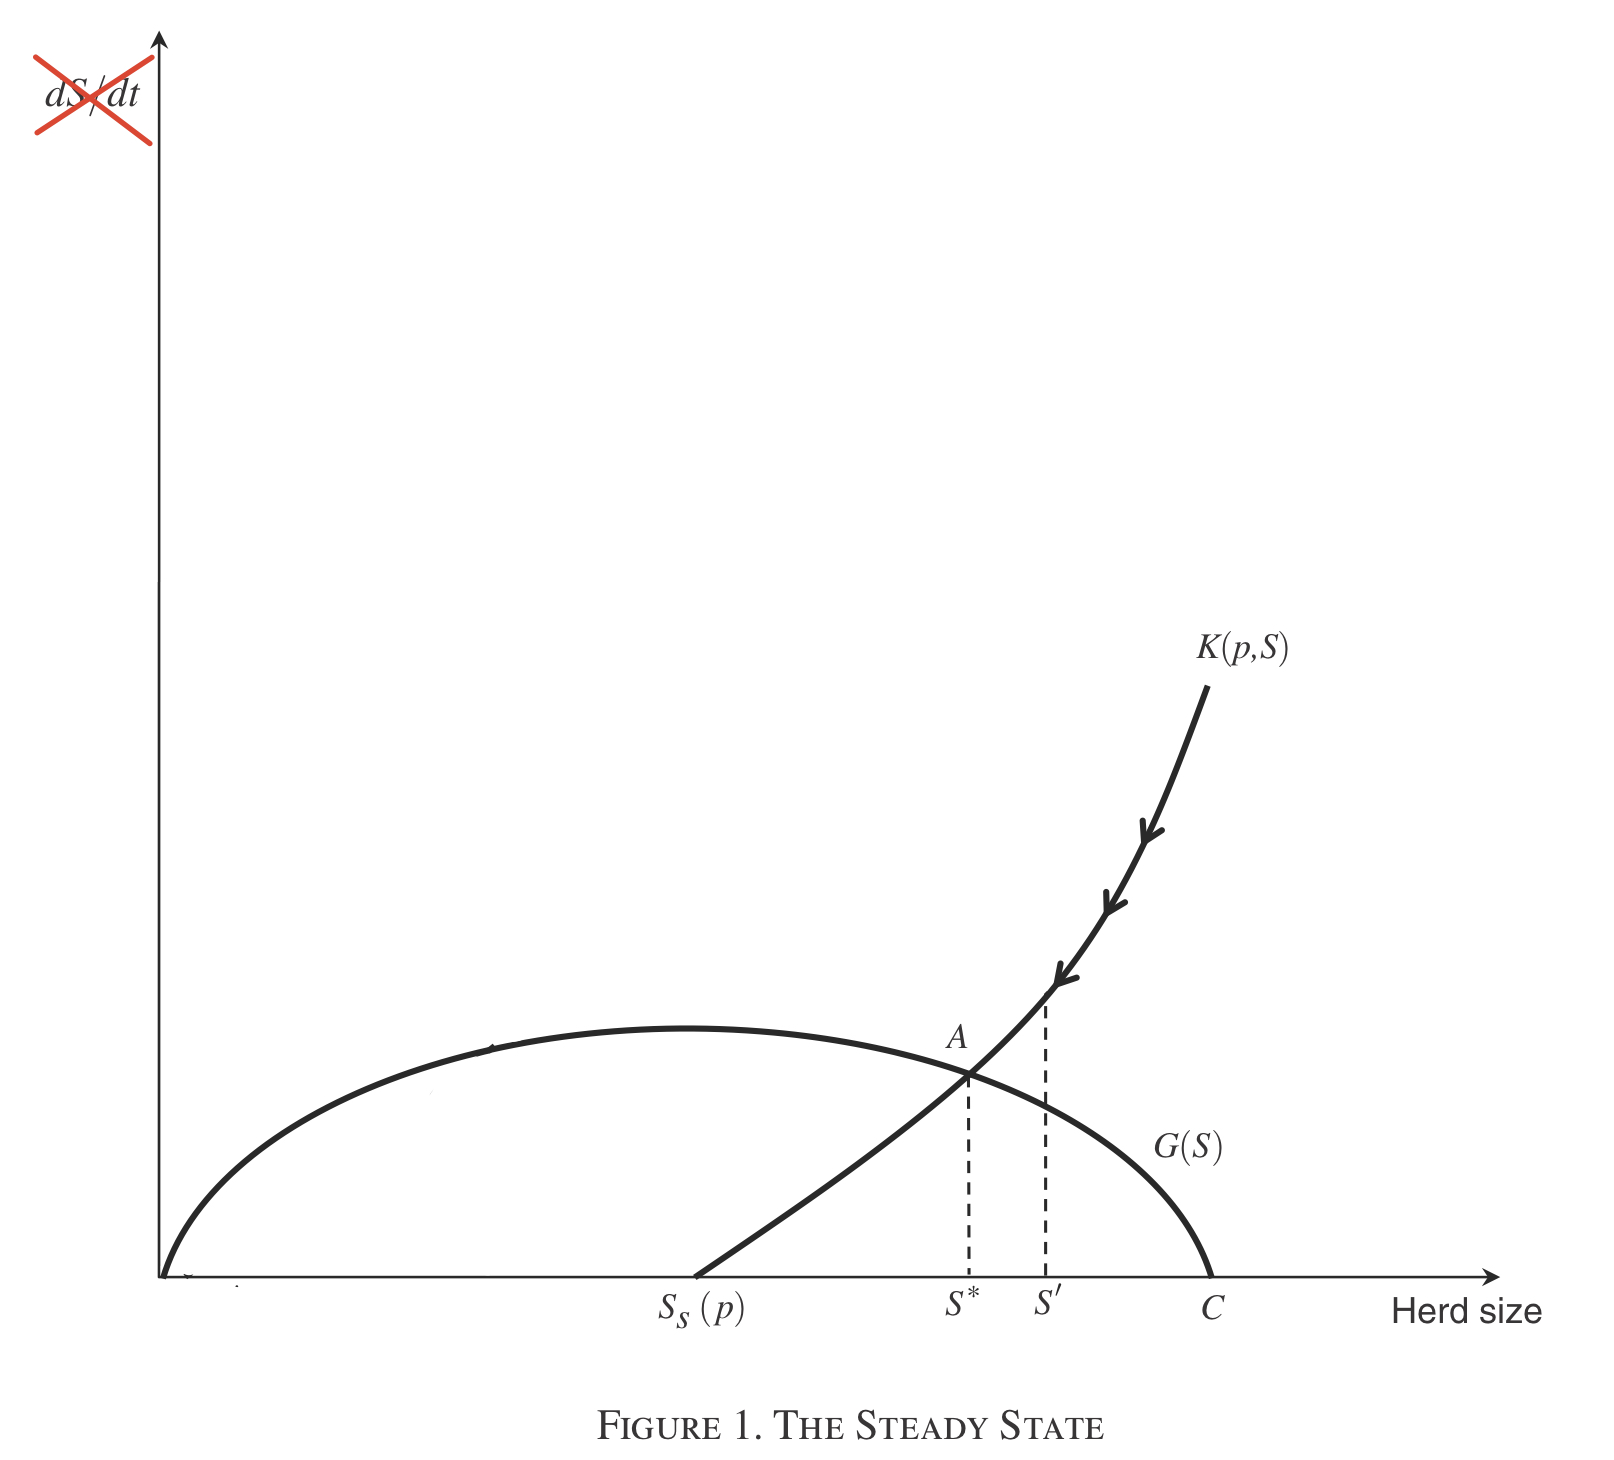
\includegraphics[width=1\textwidth]{Figure1a.jpeg}
     \begin{align*}
	\dot{S} &= G(S) - K(p, S)
\end{align*}
     \end{center}
\end{column}
\end{columns}
% DISCUSS THE KILLING FUNCTIONS
\end{frame}



% Then what happens?
%We just said we are on the green transition path of the Killing function, and slowly (by slowly I mean at the rate of 10 millions per 100 years) decreasing the herd size, but pre innovation. 
% Now, 1871, the tanning innovation in Europe increases the price one can get from a bison, because now, not only the meat, but the hide becomes very valuable. So we jump to a new killing function: the threshold \alpha^* drops, as even less skilled hunters can find it profitable to hunt, the number of hunters increase and therefore the number of killings increase.

% After the initial jump of killings, we are on the transition path, K decreases and not only do we converge towards a new steady state S*', but some hunters remain in business until we reach S_p(P') and the Herd size reaches about 100 bisons.

% To be more precise, this jump to the new killing function is both what happened for the Southern Plains, so in 1871 in reaction to the tanning innovation, as well as, 10 years later in the Northern plains, as the defeat of the Sioux nation can be modeled as an exogenous shift rightward of the distribution of hunter productivity, and the building of Northern Pacific railroad also had an effect, lowering transport costs to effectively increase profits that hunters could obtain. 

\begin{frame}
\frametitle{Proving Sufficiency Through a Model - The buffalo Hunt}
\begin{columns}
\begin{column}{0.6\textwidth}
\begin{itemize}
	\item Pre-1870: \textcolor{green}{transition path}
	\item Introduction of \textcolor{blue}{buffalo hide tanning}
	\begin{align*}
		p &\to p' & p' > p\\
		\alpha_{S'}^*(p) & \to \alpha_{S'}^*(p') & \alpha^*(p') < \alpha^*(p)  \\
		K \uparrow
	\end{align*}
	\item \textcolor{purple}{Along 1880s}
	\begin{align*}
	 	K & \downarrow & S' \to \underbrace{S^{*'} \to S_s(p')}_{\text{extinction}}
	 \end{align*} 
\end{itemize}

\end{column}
\begin{column}{0.5\textwidth} 
    \begin{center}
     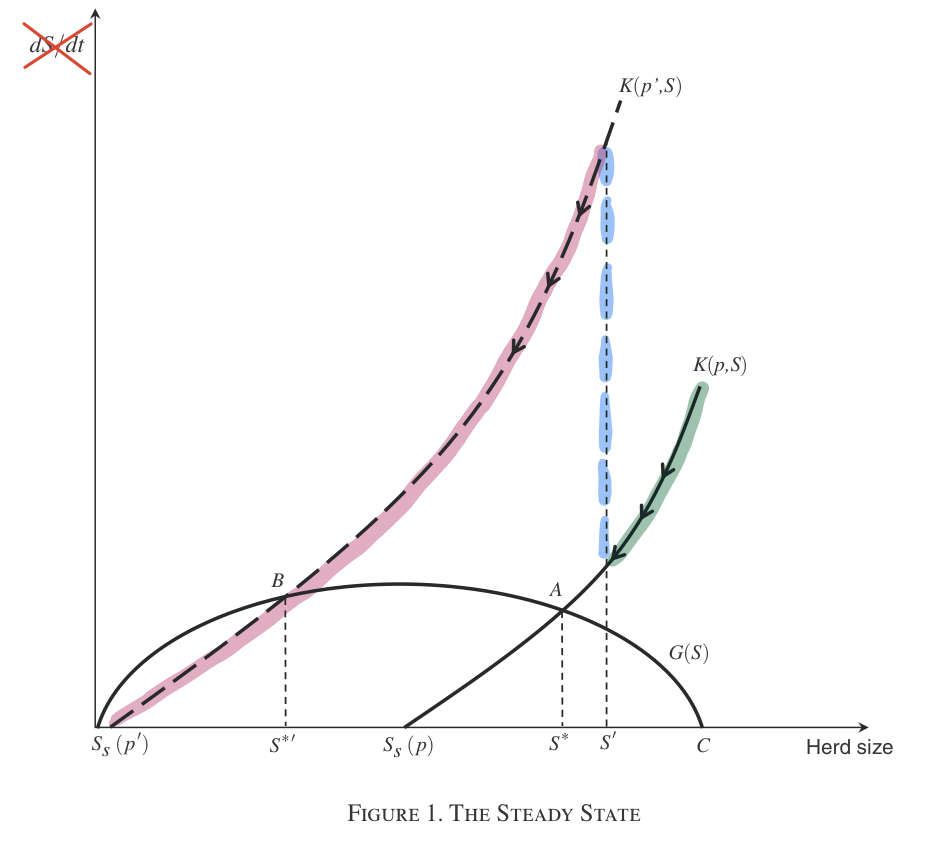
\includegraphics[width=1\textwidth]{Figure1b.jpeg}
     \begin{align*}
	\dot{S} &= G(S) - K(p, S)
\end{align*}
     \end{center}
\end{column}
\end{columns}
\end{frame}



% Is there any question at that point? 
% So now, let's move on to the second part of the demonstration, the necessity part. 
% For this, Taylor first relies on data on shipments of hides by the railroads that were collected at the time (for the reference Hornaday was a zoologist, consevationist that is credited with preserving the bison from extinction, and became the first director of what is today the Bronx Zoo).
% Taylor also, and that is definitely a contribution of the paper, builds a new dataset of import / exports of bison tides by collecting both import estimates for European countries, and by recovering export hide estimates in quite a mutistep procedure. 
% He documents this procedure quite extensively, because it is not straightforward at all to recover estimates from bison hides, in number rather than value, and to distinguish them from cattle hide, but for the interest of time, we're just gonna assume here he does a good job, and I'm gonna move to what he can get out his new data


\begin{frame}
\frametitle{Proving Necessity (0) - Building New Import/Export Data}	
Historical evidence documenting the rate of the slaughter
\begin{itemize}
	\item Data on shipments of hides by the railroads operating in Buffalo country (\textcolor{blue}{Dodge, Hornaday, Koucky late 1880s})
\end{itemize}
New data establishing the role of international trade
\begin{itemize}
	\item \textbf{Import} buffalo hide estimates for European countries.
	\item A multistep procedure to recover \textbf{export} buffalo hide estimates
\begin{enumerate}[1)]
	\item Obtain the value of US hide exports for 1865-1886.
	\item Convert hide values into hide numbers using estimates of hide prices (Warrent and Pearce price index, New York Change of Commerce reports).
	\item Eliminate cattle hides from the volume of hide export series using a model of cattle cycle.
	\item Use historical sources to motivate the key assumption that prior to 1870, and after 1886 the buffalo hide market was inexistent.
\end{enumerate}
\end{itemize}
\end{frame}

% First, he documents that exports of bison hides match, in magnitude and time, the slaughter and you can see on the left panel this jump in bison hide exports between 71 and 78-79, and then some jumps until 86, while cattle hide export estimates seem to be quite smooth.

% Second, remember that one of his conditions was that buffalo hide prices were invariant, and more precisely that they did not decrease with the increased hide supply, and this is what is shown on the right panel.

\begin{frame}
\frametitle{Proving Necessity (1) - Documenting the Assumptions}
\begin{columns}
\begin{column}{0.5\textwidth}  %%<--- here
\textbf{A consistent timeline}
    \begin{center}
     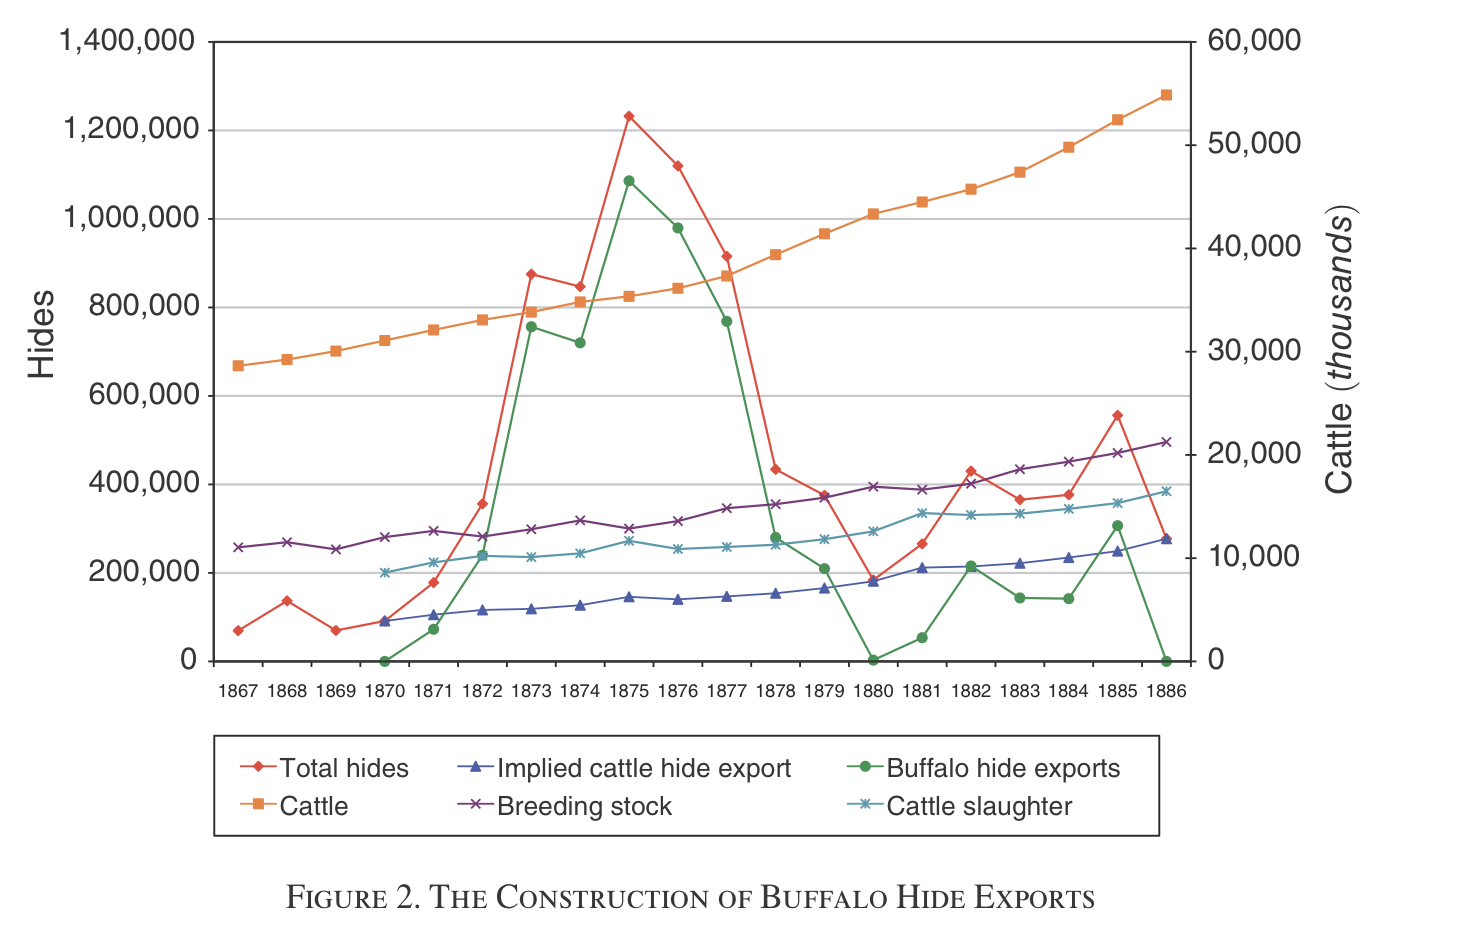
\includegraphics[width=1\textwidth]{Figure2_exports.jpeg}
     \end{center}
\end{column}
\begin{column}{0.5\textwidth}
\textbf{Invariant buffalo hide prices}
\begin{center}
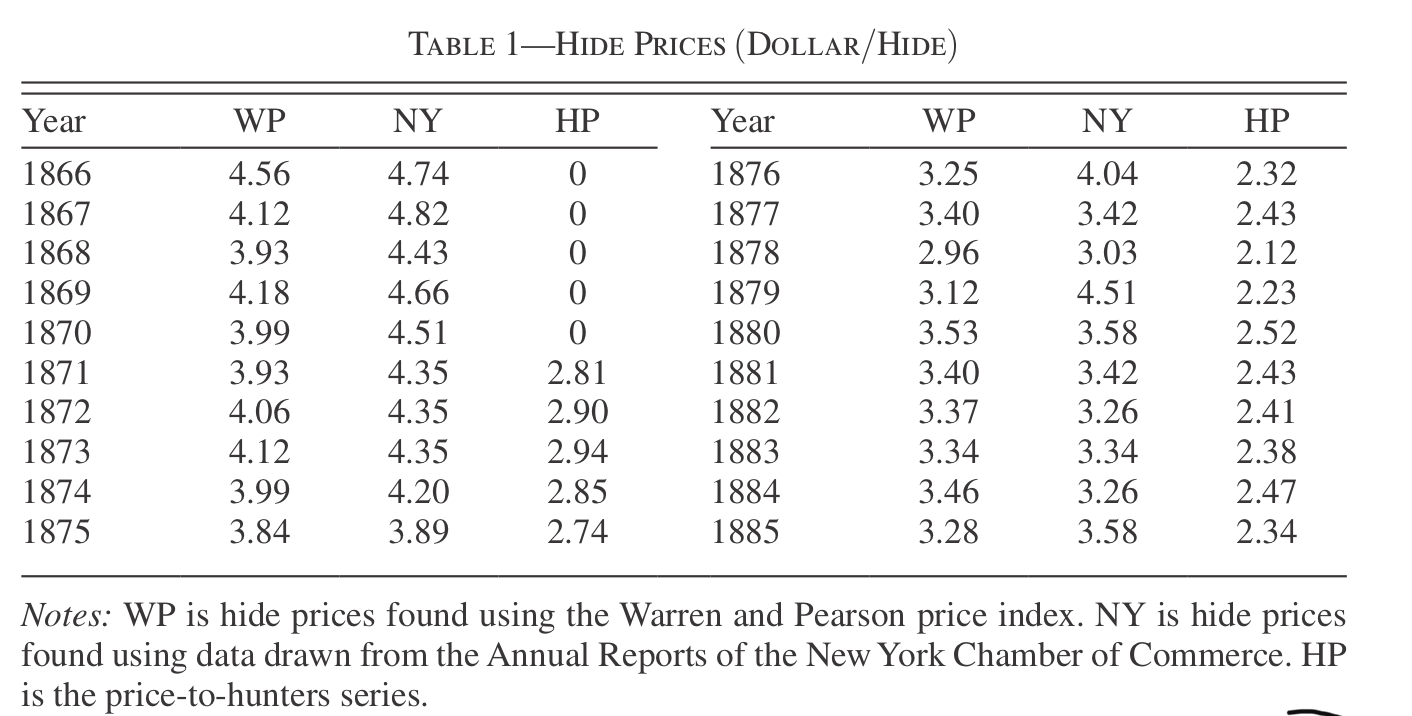
\includegraphics[width=1\textwidth]{Table1.jpeg}	
\end{center}	
\end{column}
\end{columns}
\end{frame}

% The economic mechanism behind is that if cattle and buffalo hides are perfect substitutes, and US buffalo supply is small relative to the total number of hides transacted in world market, then the increased supply of US buffalo hides should not affect world prices. This is what he seems to find in his data, using variation in the price of tanned sole leather, and estimates that in 1975 buffalo hides were at most 4% of total world hide exports.


\begin{frame}
\frametitle{Proving Necessity (1) - Documenting the Assumptions}
\begin{columns}
\begin{column}{0.5\textwidth}  %%<--- here
\begin{itemize}
	\item Cattle \& buffalo hides are perfect substitutes
	%\begin{itemize}
	%\item Variation in the price of tanned sole leather
	%\end{itemize}
	\item US buffalo supply is small relative to the total number of hides transacted in world markets (3-4 \% at peak)
	%\begin{itemize}
	%	\item 1875 (peak year): \\ buffalo hides $=3-4\%$ of total world hide export
	%\end{itemize}
\end{itemize}\end{column}
\begin{column}{0.5\textwidth}
\textbf{Invariant buffalo hide prices}
\begin{center}
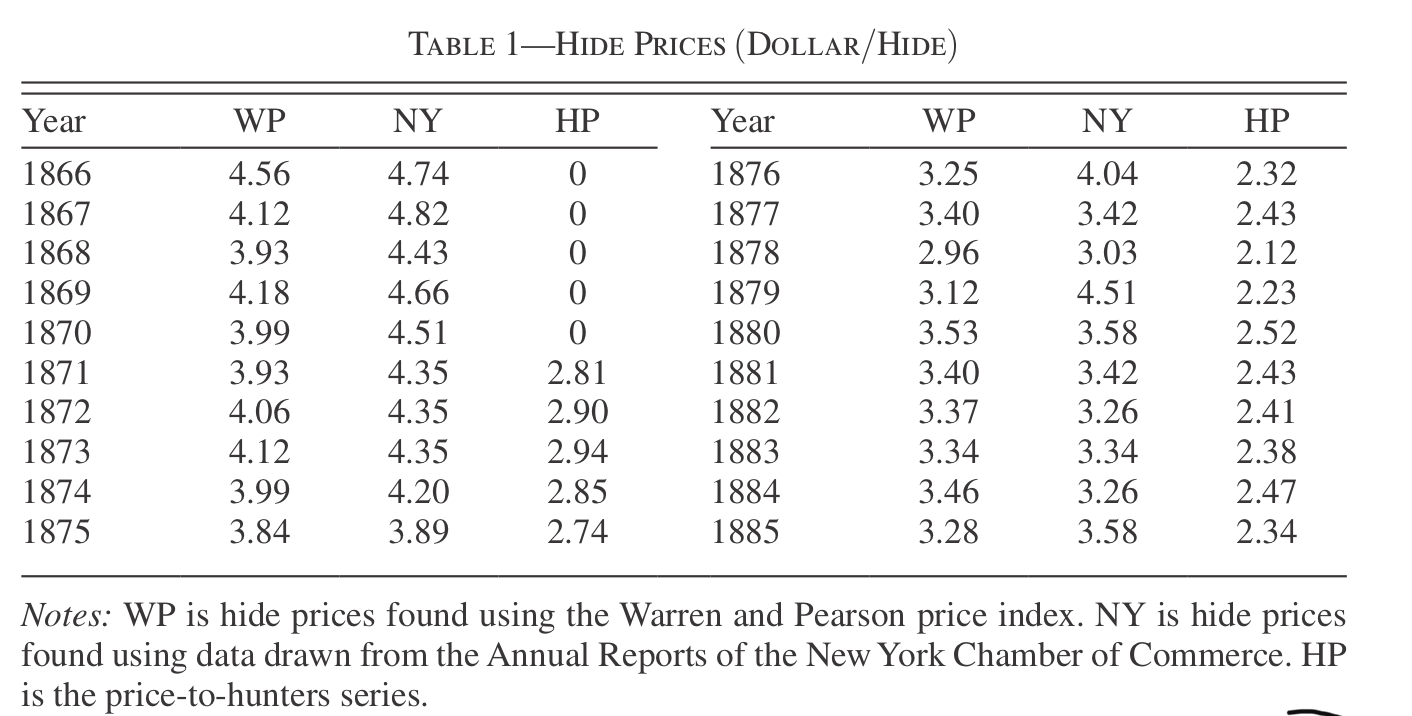
\includegraphics[width=1\textwidth]{Table1.jpeg}	
\end{center}	
\end{column}
\end{columns}
\end{frame}


% Taylor also needs to show that the increase in hide exports is not just a European Demand shock, or just a US cattle supply shock. To do so, he treats the innovation as a quasi-experiment, with Canada as the ontrol county with no ability to tan buffalo hides, and the UK and France as treatment countries with the ability to tan. It assumes that innovation assignment was exogenous. 
%s_it: the US share of raw hide imports in total raw hide imports into country i (France, UK, Canada) in year t (1866-1887)
%\alpha_i Country FE
%\beta_it Country time trend
%T_it^s Treatment effect = 1 during 1872-1879 (Southern)
%T_is^S Treatment effect = 1 during 1881-1886 (Northern)
%Note that the absence of positive statistically coefficients for the France and UK intercepts are evidence against a European Demand Shock. Taylor argues that the positive and huge coefficient for Canada is explained by the fact that Canada is very close to the US.
% Finally it's worth commenting the difference in magnitudes and statistical significance of the South vs North treatment periods: as the innovation seems to have driven exports really in the 70s. 
% A potential explanation could be that, then, the innovation spread to the US.

\begin{frame}
\frametitle{Proving Necessity (2) - Exploiting a Quasi-experiment}
\begin{columns}
\begin{column}{0.3\textwidth}
\begin{align*}
	s_{it} &= \alpha_i + \beta_i t + \gamma T_{it}^S + \delta T_{it}^N + \epsilon_{it}
 \end{align*}	
\footnotesize{
Rulling out \\
- a US Supply Shock to Cattle Production
\\
- a European Demand Shock}
\end{column}
\begin{column}{0.7\textwidth}
\begin{center}
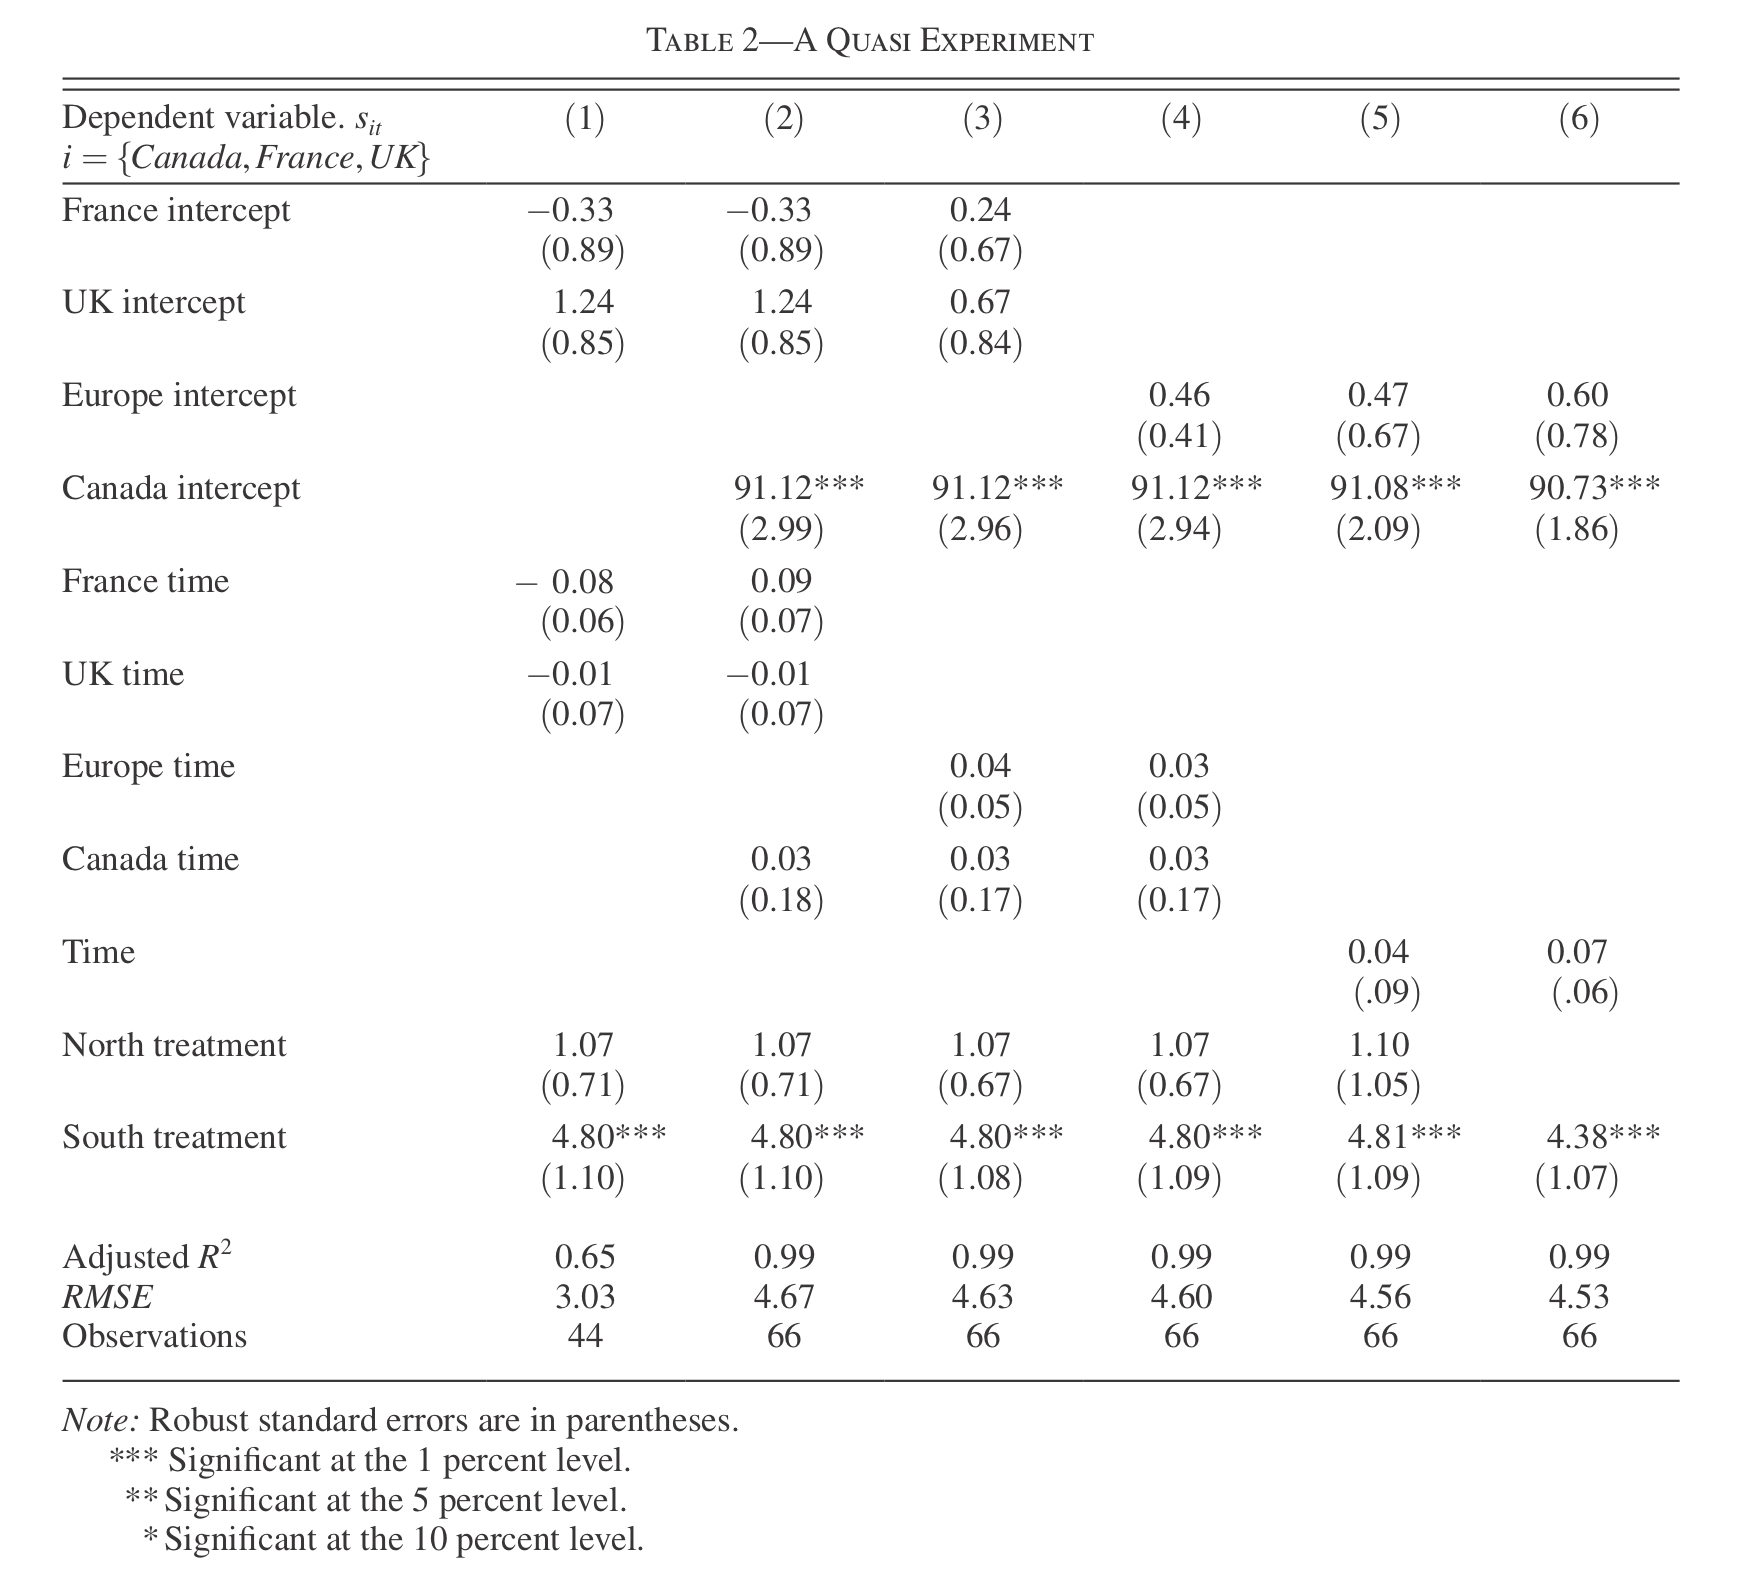
\includegraphics[width=0.9\textheight]{Table2.jpeg}
\end{center}	
\end{column}
\end{columns}
\end{frame}


% Finally, in order to prove the necessity of his mechanism, Taylor tries to rule out the alternative hypotheses I mentioned before, and I saw a few comments of people who thought this part was more or less convincing.

\begin{frame}
\frametitle{Proving Necessity (3) - Rulling out Alternative Hypothesis}
\begin{enumerate}[a)]
	\item The Army and Federal Government Story
	\item The Railroads Story
	\item The Environmental Change and Native Overhunting Story
\end{enumerate}
\end{frame}




% Finally, and this is my last slide, I'd like to relate how this paper could be "adapted" to what I call a "local rush" but really because I couldn't figure out how to say it differently. More precisely, I think this paper does a good job at showing different consequences international trade can have on local markets, by making a local catastrophe into a simple minor event on the world stage.
%These roles go from technology diffusion, limiting price adjustment, therefore masking scarcity signals that markets would usually use to adjust. As well as potentially altering incentives for environmental regulation.



\begin{frame}
\frametitle{Conclusion : The role of International Trade}
By making [your favorite local rush] a minor event on the world stage, international trade plays a role as a mechanism...
%being small on world markets meant that some o the typical insulating and signaling properties provided by a market price system were missing
\begin{enumerate}
	\item ... bringing advanced foreign technology to local markets
	\item ... limiting price adjustment and masking scarcity signals
	\begin{itemize}
		\item Buffalo hide prices did not decrease with increased supply
	\end{itemize}
	\item ... increasing the likelihood of extreme events (\textcolor{blue}{Copeland and Taylor 1999}) 
	\item ... altering the incentives for environmental regulation (\textcolor{blue}{McAusland 2003, 2008})
	\begin{itemize}
		\item A bison export tax would be born entirely by the domestic hide hunters
	\end{itemize}
\end{enumerate}
\end{frame}

	


\end{document}